\chapter{Einleitung}
\lhead{Einleitung}
Das Mooresche Gesetz hat in den letzten vierzig Jahren zu einem
exponentiellen Wachstum der verf"ugbaren maschinellen Rechenleistung
gef"uhrt und damit ein goldenes Zeitalter der Anwendung numerischer
Modelle in allen Wissenschaftszweigen gef"uhrt.
Ein eigenes Studienfach ``Computational Science'' ist geschaffen worden,
um der gewachsenen Bedeutung von Computer-Simulationen Rechnung zu
tragen. Und die Konsequenzen sind vielfach sp"urbar.
Numerische Simulation von Str"omungen hat aerodynamische Messungen
im Windkanal ersetzt.

Um ein gegebenes numerisches Problem zu l"osen, ist eine bestimmte
Anzahl von Gleit\-komma-Operationen durchzuf"uhren.
Bis zum Ende das zwanzigsten Jahrhunderts dominierte der Zeitaufwand f"ur
die Gleitkommaoperationen die "ubrigen Instruktionen.
Zu Beginn der Computer-"Ara mussten Gleitkomma-Operationen in Software
implementiert werden, weil Prozessoren nur Ganzzahloperationen 
beherrschten. Mit der Entwicklung von Hardware-Gleitkommaprozessoren
und deren Integration in Standardprozessoren war die Auf"uhrungszeit
f"ur Gleitkomma-Operationen an die Prozessor-Taktrate gekoppelt.
Die Rechen-Leistung wuchs daher mit der Taktrate
(Abbildung~\ref{processorperformance}).
\begin{figure}
\begin{center}
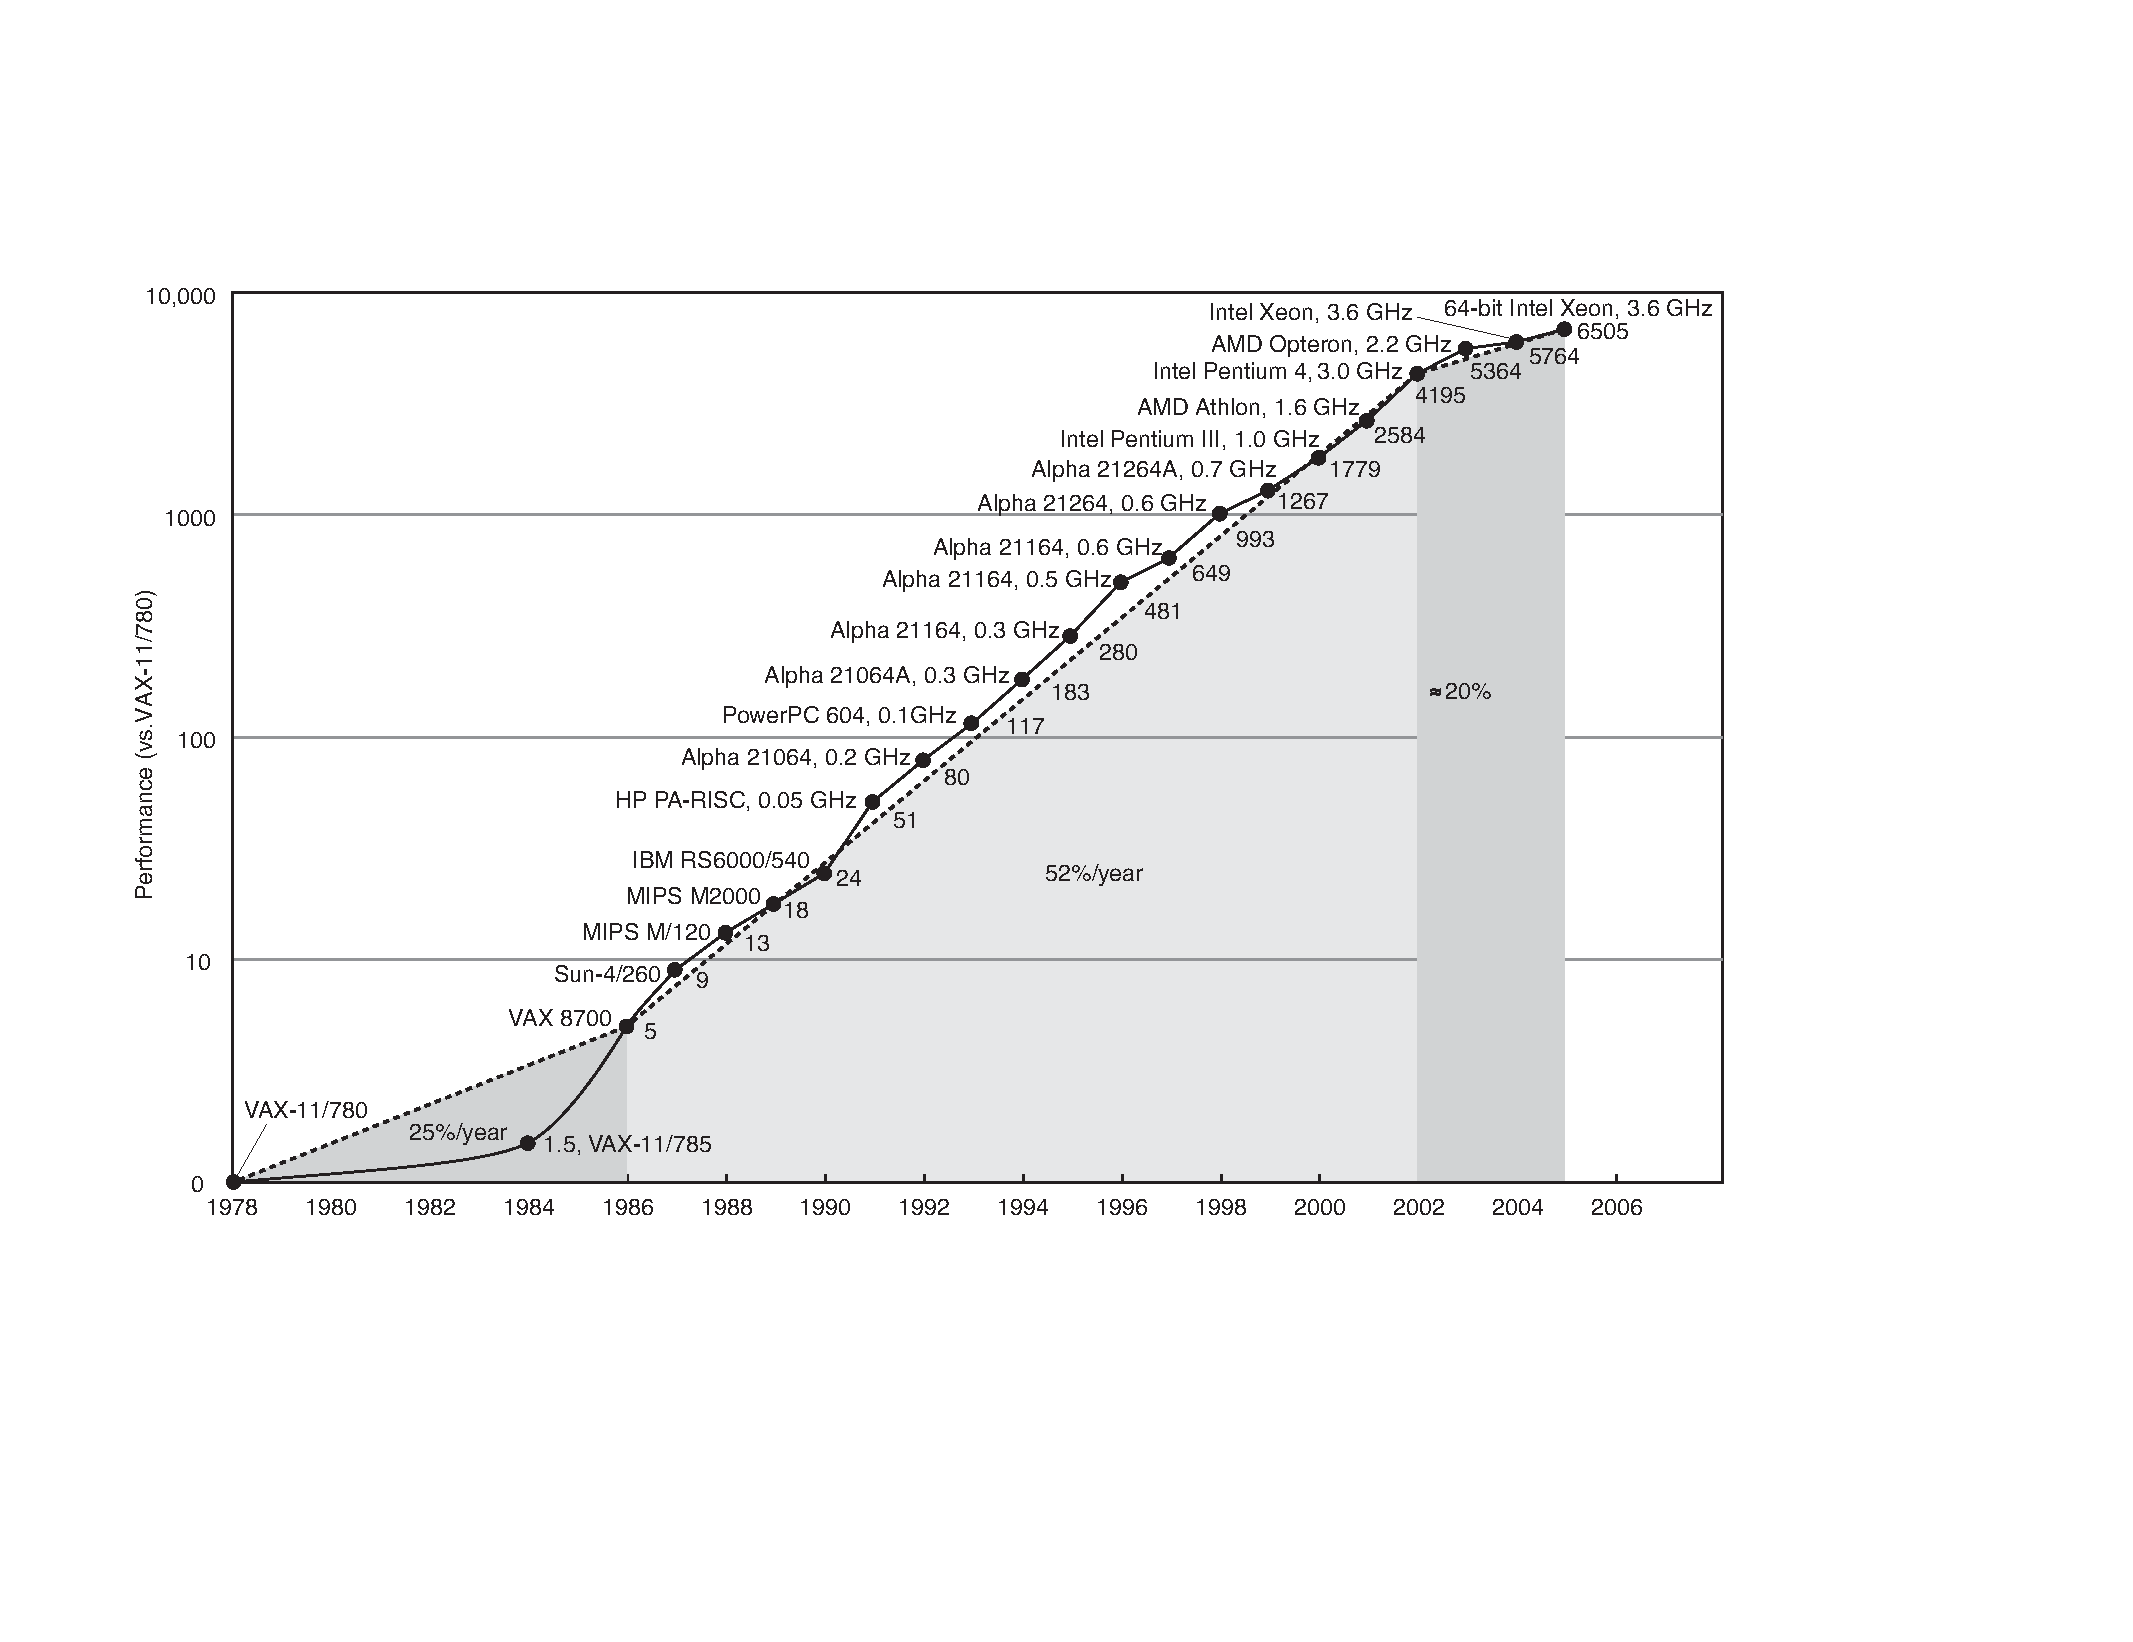
\includegraphics[width=\hsize]{images/processorperformance.pdf}
\end{center}
\caption{Prozessorleistung basierend auf SPEC relativ zu einer VAX-11/780}
\label{processorperformance}
\end{figure}

Grosse numerische Simulationen verlangen aber nicht nur eine grosse
Menge von Rechenoperationen, sondern auch eine grosse Zahl von
Zahlen, die miteinander verkn"upft werden m"ussen.
Mit wachsendem Umfang der Simulationen wurde daher auch mehr
und mehr Speicher notwendig. Schneller Speicher (statisches RAM) ist
zu teuer und verbraucht zuviel Energie. Grosse Speicher verwenden
daher dynamisches RAM. Zu Beginn der Mikroprozessor-"Ara war
die Prozessortaktrate mit der Zykluszeit des dynamischen RAM
vergleichbar, ein Prozessor konnte in jedem Taktzyklus ein
Element ein Wort aus dem dynamischen RAM lesen. Die Prozessortaktraten
entwickelten sich jedoch deutlich schneller als die DRAM-Zykluszeiten
(Abbildung~\ref{memorywall}).
\begin{figure}
\begin{center}
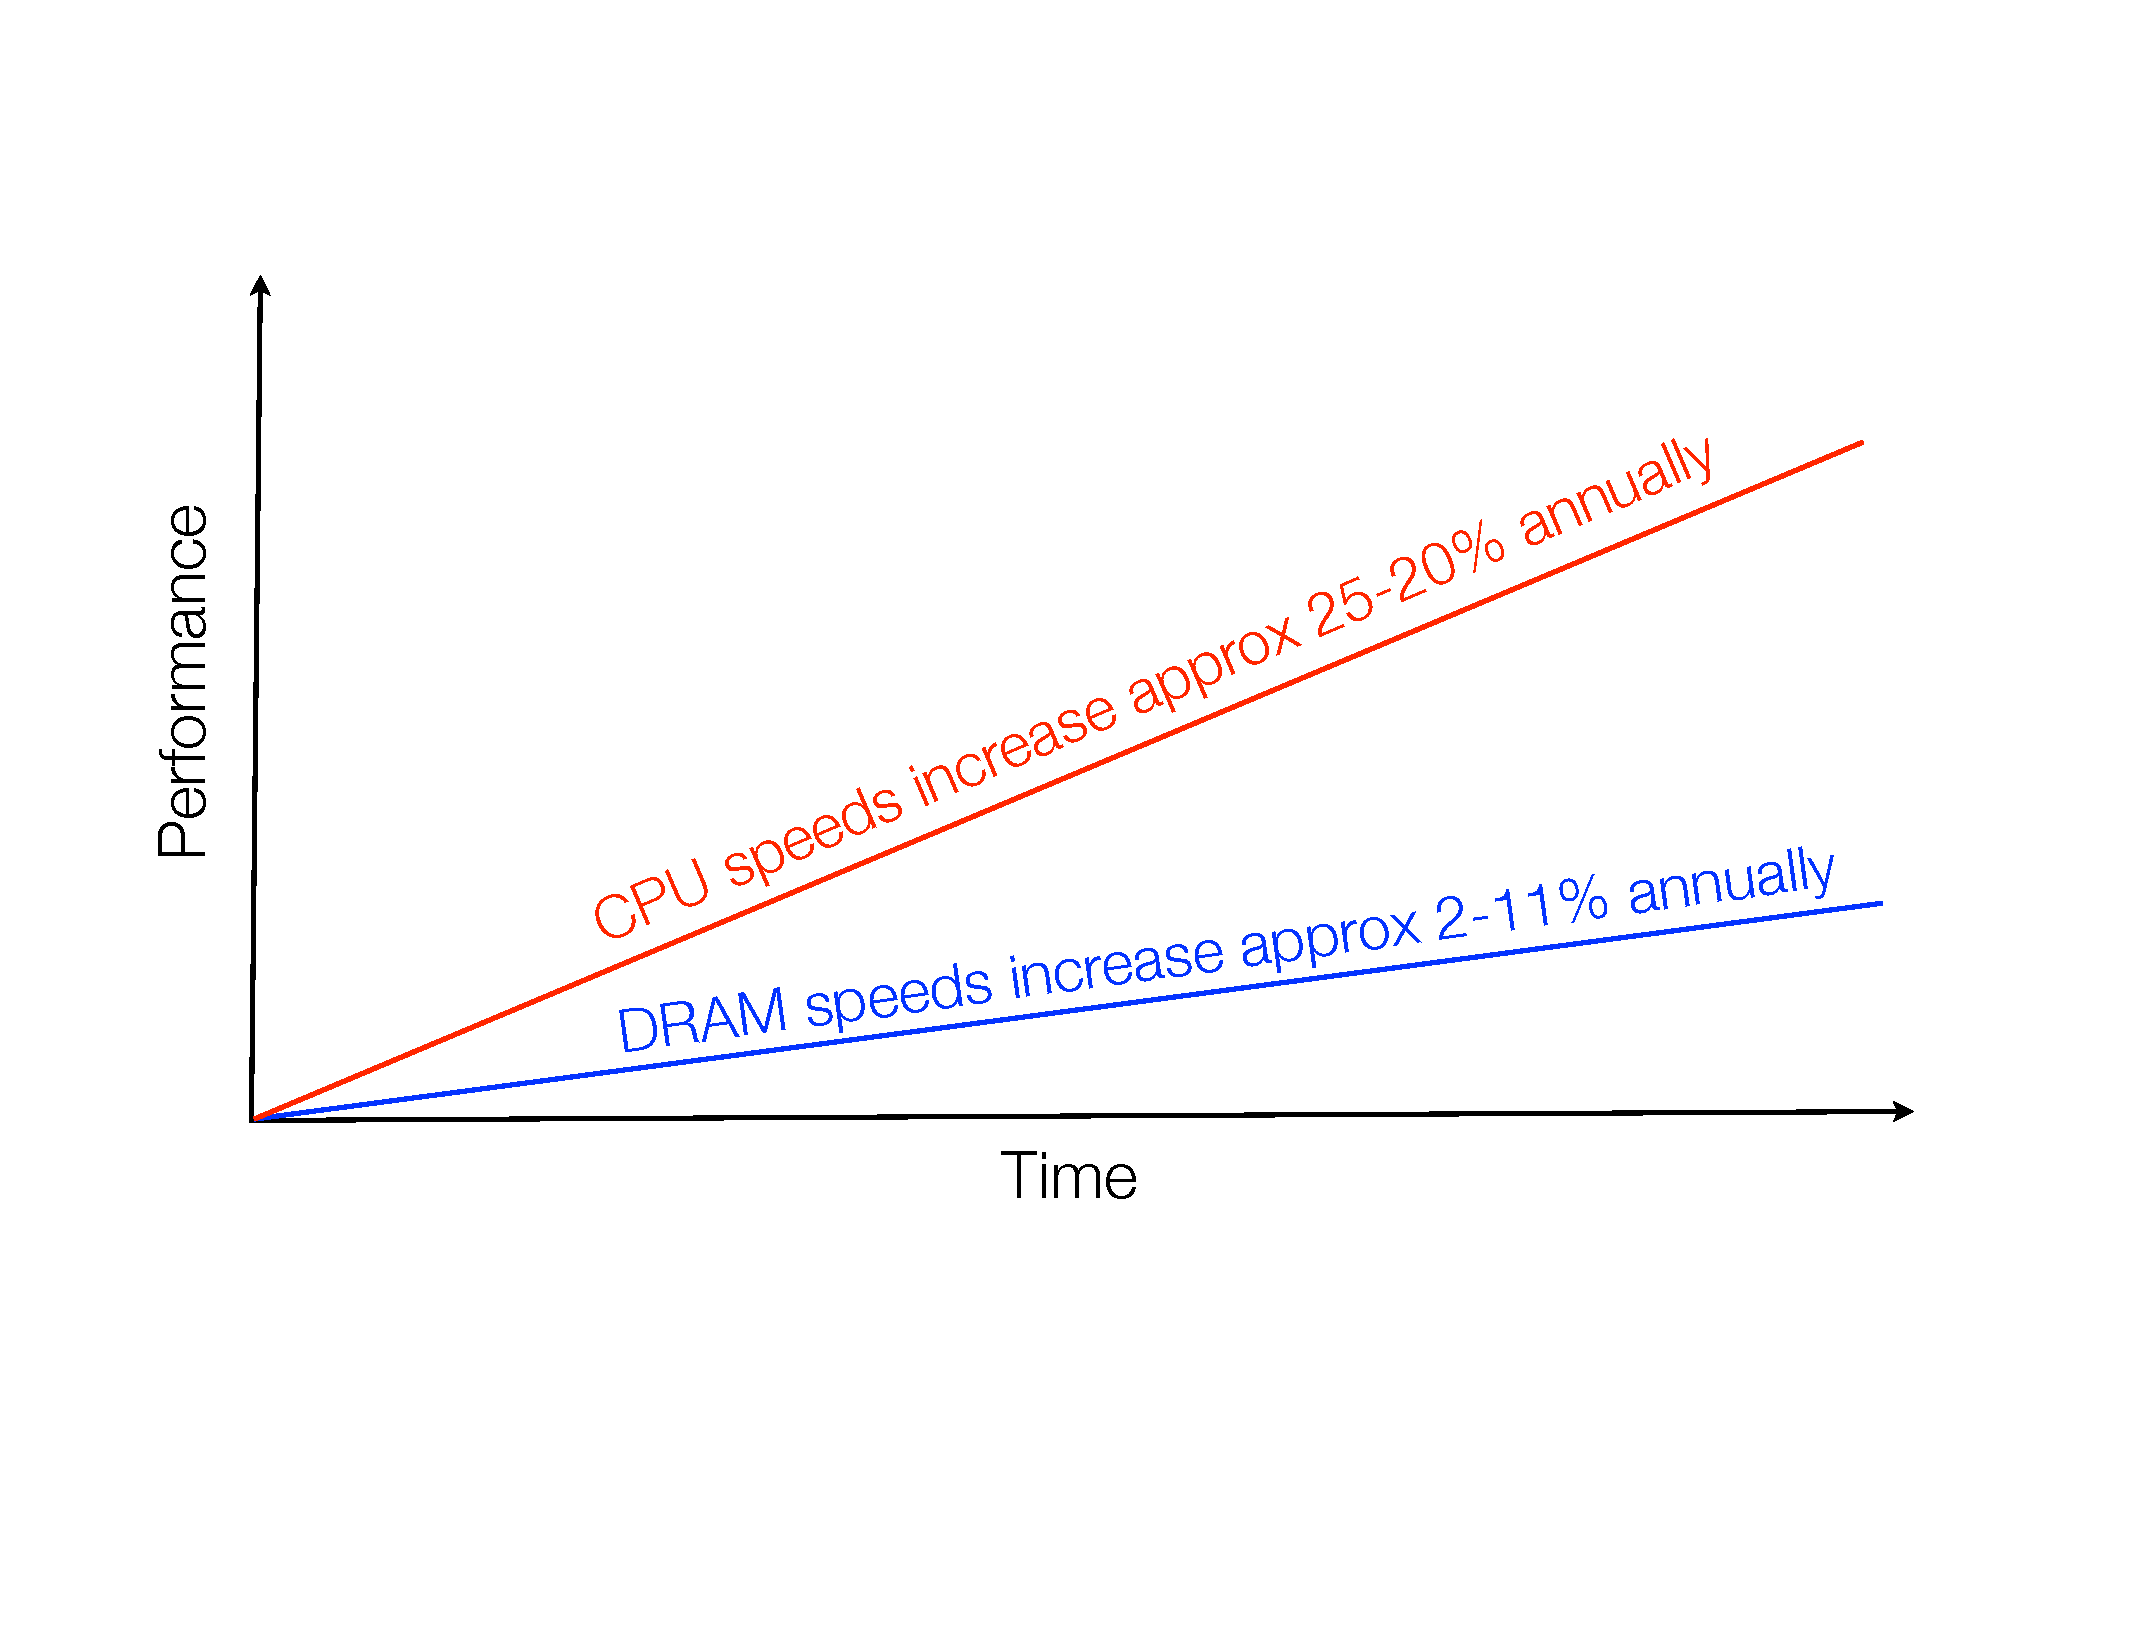
\includegraphics[width=0.6\hsize]{images/memorywall.pdf}
\end{center}
\caption{Entwicklung von Prozessor- und Memory-Performance
\label{memorywall}}
\end{figure}

Ein Teil der Performance-L"ucke kann durch
die Breite des Memory-Bus kompensiert werden. So hatten zum Beispiel die
Enterprise-Systeme von Sun Microsystems in den sp"aten Neunziger-Jahren
einen 1024-bit breiten Memory-Bus, vier mal breiter als was die meisten
Desktop-Mikroprozessor-System in dieser Zeit hatten.
Diesem L"osungsansatz setzt die Schaltungskomplexit"at jedoch enge Grenzen.

Eine Hierarchie von Caches verschiedener Gr"osse und abnehmender
Geschwindigkeit passt in modernen Systemen den relativ langsamen
Hauptspeicher an den schnellen Prozessor an. Dies funktioniert,
wenn Software Instruktionen und Daten immer wieder benutzt.
Tats"achlich trifft dies f"ur viele Betriebssysteme, Benutzeroberfl"achen
und Awendungssoftware in hohem Mass zu.
Sobald jedoch grosse Datenmengen verarbeitet werden m"ussen kann
es sehr leicht geschehen, dass die Daten nicht in einen Cache passen,
oder nur sehr sporadisch gelesen werden, so dass kaum ein Zugriff
vom Caching profitieren kann.
In diesem Fall beginnt sich das System so zu verhalten, als w"aren die
Caches gar nicht vorhanden.

Caches f"uhren zu dem Problem, dass Cache und Hauptspeicher konsistent
gehalten werden m"ussen. Die daf"ur notwendige Hardware limitiert die
Anzahl Prozessoren, die zu einem System verbunden werden k"onnen.
Mehr als wenige hundert Prozessoren k"onnen nicht integriert werden.
Solch grosse Systeme bestehen aus vielen einzelnen Systemboards, die
untereinander verbunden sind. Es ist klar, dass der Datenaustausch
innerhalb eines Systemboards schneller ist als der Datenaustausch
"uber Systemboards hinweg.

\begin{figure}
\begin{center}
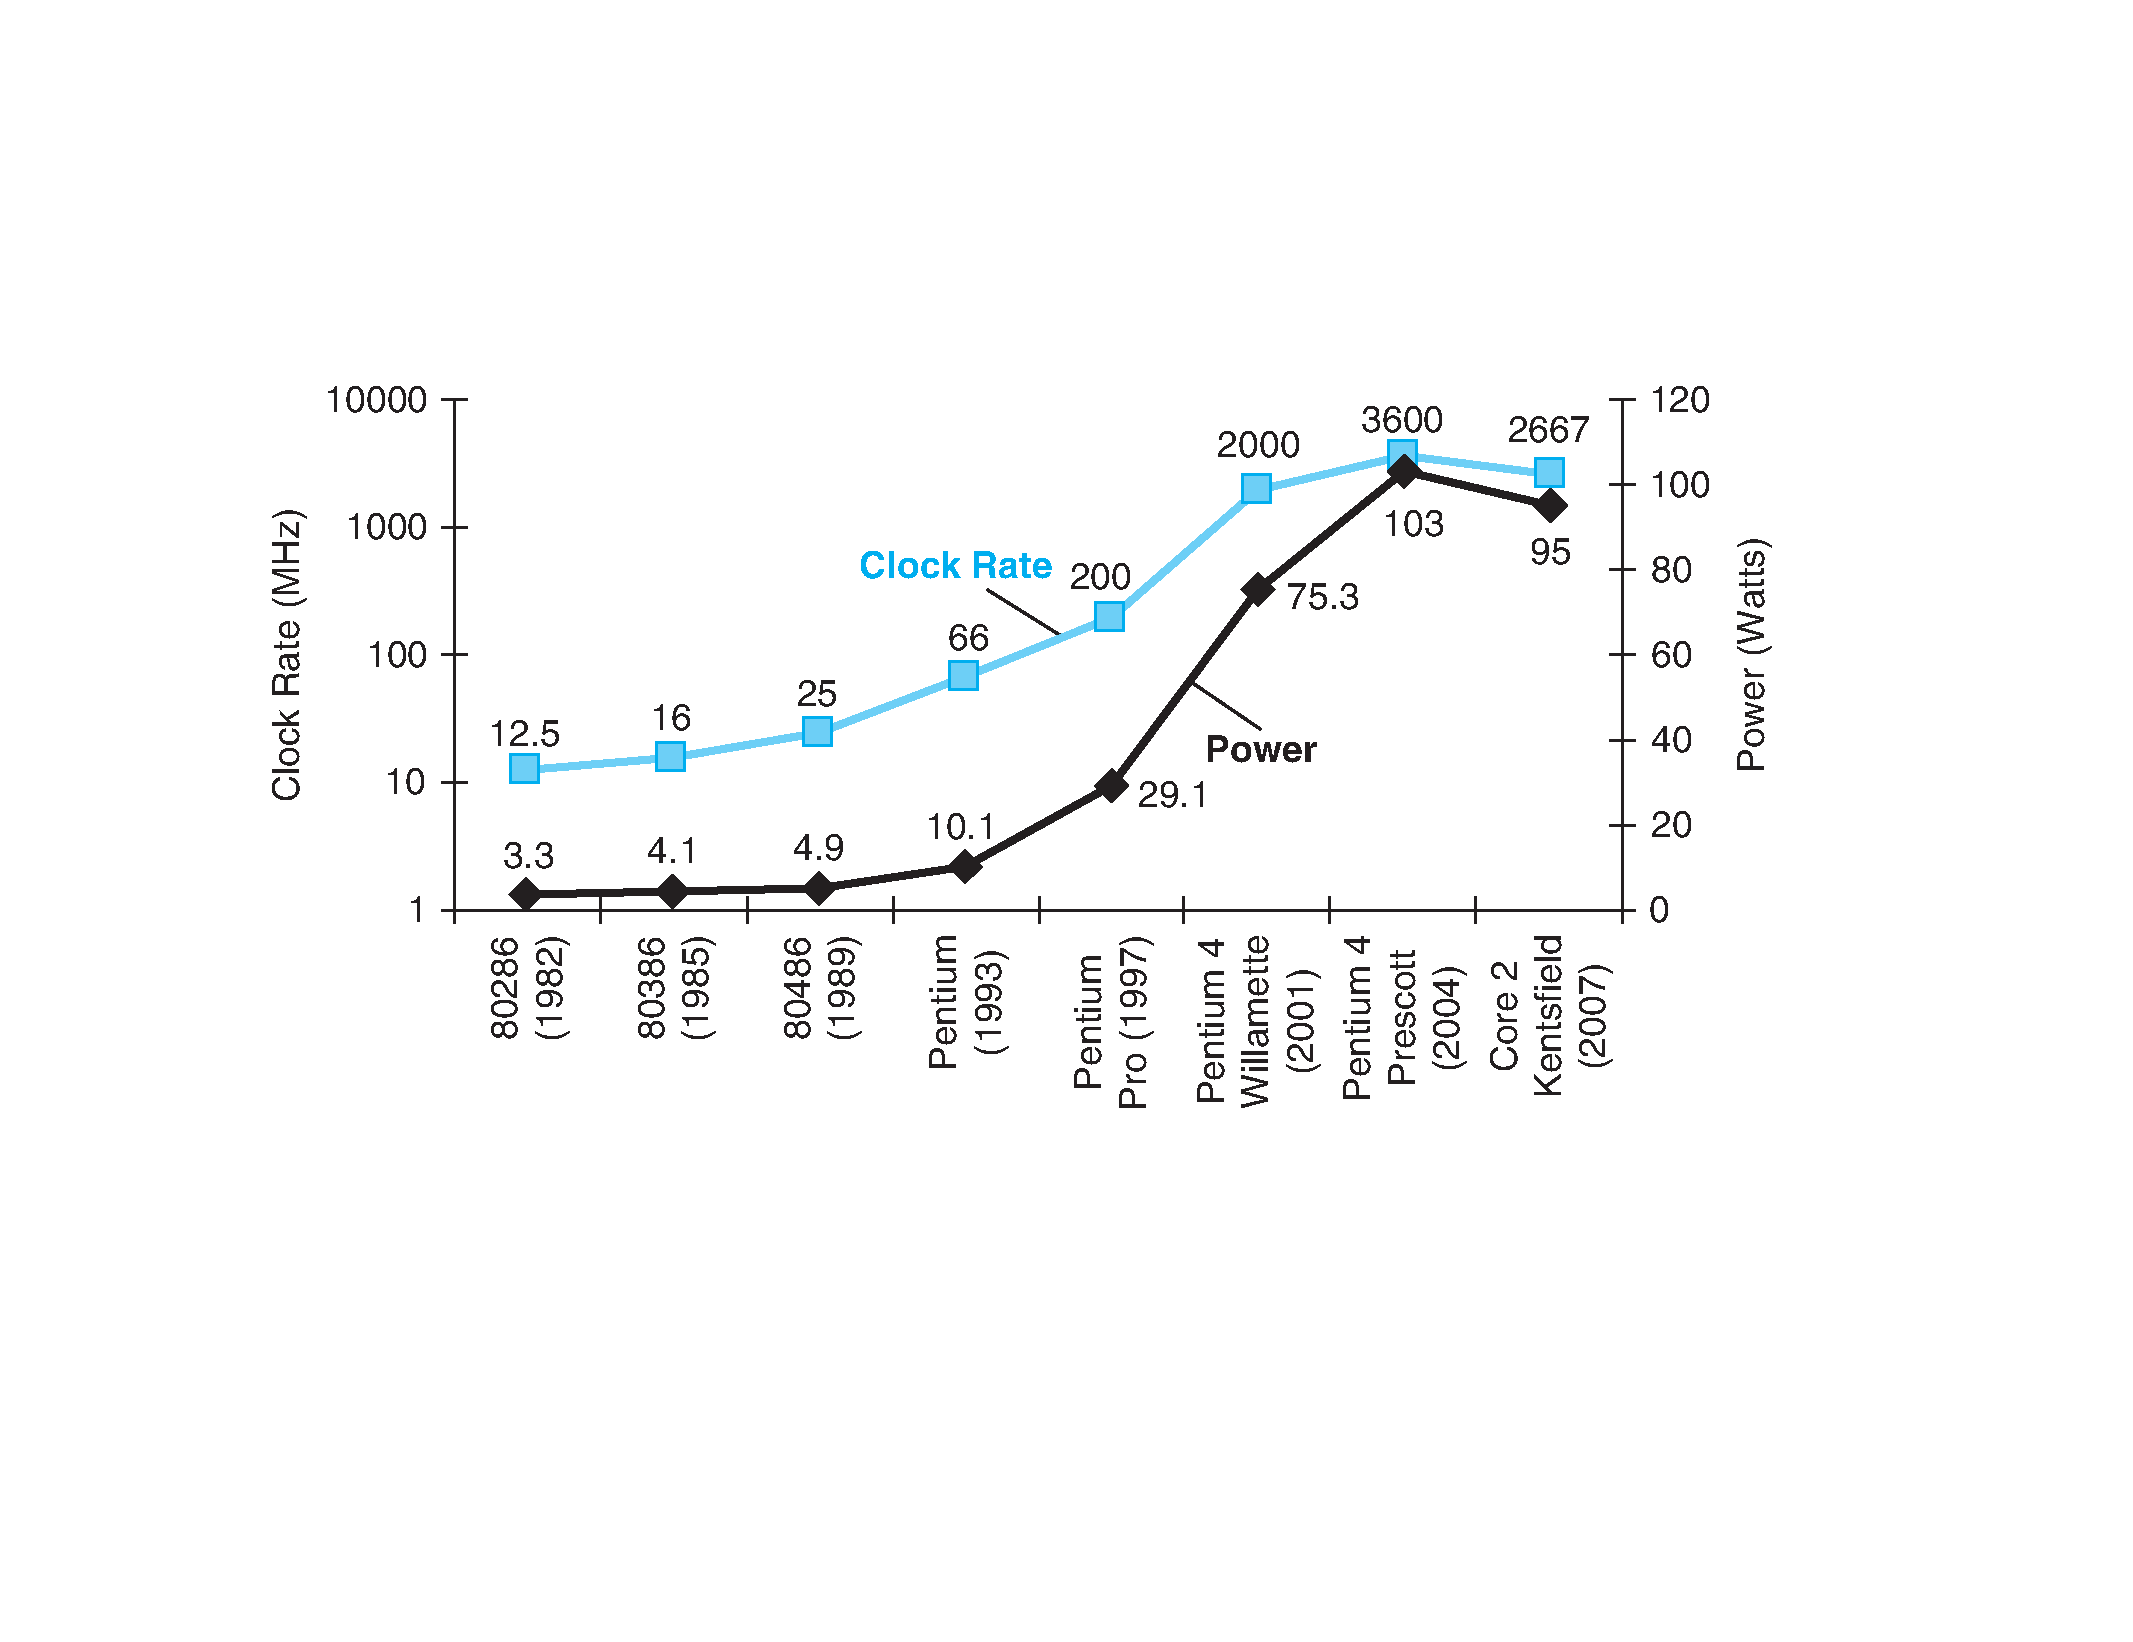
\includegraphics[width=\hsize]{images/powerwall.pdf}
\end{center}
\caption{Leistung limitiert die Taktrate\label{powerwall}}
\end{figure}
Im 21.~Jahrhundert zeichnete sich ab, dass sich die Taktrate kaum mehr
weiter steigern l"asst, der Aufwand, die Verlustleistung der Prozessoren
abzuf"uhren, wurde zu gross.
Die Fortschritte in der Prozessor-Herstellung werden daher in 
j"ungster Zeit nicht mehr f"ur die Steigerung der Taktrate
verwendet, sondern zur Integration mehrere Cores auf einem
einzigen Chip.
Will man die Taktrate eines Prozessors zu verdoppeln, muss man
bei gleicher Technologie ungef"ahr
die vierfache Verlustleistung abf"uhren. Integriert man stattdessen
vier Cores auf einem Chip, wird die Verlustleistung ebenfalls 
vervierfacht, aber die zur Verf"ugung stehende Rechenleistung
wird ebenfalls vervielfacht. Die Cores eines Chips teilen sich
den Memory-Bus, auch dies limitiert die n"utzliche Anzahl Chips.

Moderne Prozessoren integrieren zwar eine grosse Zahl von Cores auf
einem Chip, doch f"ur die Gr"ossenordnung aktueller numerischer
Probleme immer noch viel zu wenige. F"ur solche Probleme geeignete
Systeme m"ussen daher aus einer grossen Zahl von einzelnen Prozessoren
zusammengebaut werden. 

Die eben skizziierte Entwicklung der Chip-Technologie liefert die
Rahmenbedingungen f"ur massive numerische Simulationen, die in diesem
Seminar untersucht werden sollen.
\begin{enumerate}
\item {\bf Massiv parallel:} Nur durch Einsatz einer sehr grossen Zahl
von Prozessoren kann gen"ugen Rechenleistung akkumuliert werden.
\item {\bf Massiv cache-basiert:} Nur durch massiven Einsatz von
Caches kann sichergestellt werden, dass die Prozessoren ausreichend
mit Daten versorgt werden.
\item {\bf Nicht uniformer Speicherzugriff:} Ein System mit
sehr vielen Prozessoren kann mit uniformem Speicherzugriff gebaut
werden.
\end{enumerate}
Ziel dieses Seminars ist daher, mathematische Methoden und geeignete
Algorithmen zu deren Umsetzung kennenzulernen. Dabei geht es weniger
darum, irgendwelche Rekorde zu knacken, sondern an Beispielen zu
lernen, wie man mit den genannten Schwierigkeiten umgehen kann.
In den nachfolgenden Kapiteln werden daher einzelne Aspekte etwas
vertieft untersucht:
\begin{enumerate}
\item[2.] Performance-Aspekte moderner Maschinen.
\item[3.] Software-Hilfsmittel zur Implementation von parallelen Algorithmen
\item[4.] Datenverwaltung
\item[5.] Eine Auswahl gut geeigneter paralleler Algorithmen
\end{enumerate}
